\documentclass{beamer}
\setbeamertemplate{navigation symbols}{}

% Varia a cor da applet  (posso mudar aqui a cor)
%\usetheme{Antibes}
%\usetheme{Copenhagen}
%\usetheme{Darmstadt}
%\usetheme{JuanLesPins}
%\usetheme{Hannover}
\usetheme{PaloAlto}
%\usecolortheme{beaver}
\useoutertheme{infolines}
\usefonttheme[onlylarge]{structurebold}

\setbeamerfont{frametitle}{size=\normalsize,series=\bfseries}
\setbeamertemplate{navigation symbols}{} 

%definio dos packages
\usepackage{color}
\usepackage[english]{babel}
\usepackage[latin1]{inputenc}
\usepackage{graphics}
\usepackage{graphicx}
\usepackage{epsfig}
\usepackage{hyperref}
\usepackage{url}
\usepackage{breakurl}
\usepackage{enumerate,rotating}
\usepackage{times}
%\usepackage{multimedia}
\usepackage{movie15}
\usepackage{amsmath}
\usepackage{amssymb}
\usepackage{tikz}
\usepackage{array}
\usepackage{multirow}
\usepackage{color}

\newcommand\tab[1][1cm]{\hspace*{#1}}
\definecolor{mycolor}{rgb}{0.2,0.5,0.9}

\tikzstyle{block}=[draw opacity=0.7,line width=1.4cm]

%configura��o da p�gina principal(titlepage)
%\title{TouchAll}
\title[TUI]{TUI (formerly TouchAll)}
\subtitle{A Multi-Touch, Gestures, and fiducials Framework for ActionScript 3.0}
\author[G. Amador\\ \& \\A. Gomes]{
\texorpdfstring{
	\begin{columns}
		\column{.45\linewidth}
		\centering
		G. Amador\\
		\href{mailto:g.n.p.amador@gmail.com}{g.n.p.amador@gmail.com}
		\column{.45\linewidth}
		\centering
		A. Gomes\\
		\href{mailto:agomes@di.ubi.pt}{agomes@di.ubi.pt}
	\end{columns}
}\\
\vspace{1cm}
Videos: \url{https://goo.gl/eZ90NI}\\
Source code: \url{https://goo.gl/Ue2ICZ}
}
%\addtobeamertemplate{title page}{}{
%\begin{center}
%$\;$\\ Videos: \url{https://goo.gl/eZ90NI}
%$\;$\\ Source code: \url{https://goo.gl/Ue2ICZ}\\
%\end{center}}
\date{\today}

\begin{document}

%\AtBeginSection[]
%{
%	\begin{frame}[allowframebreaks]
%	\frametitle{Tabela de Conte�dos}
%	\tableofcontents[currentsection,hideothersubsections]
%	\end{frame}
%}
%
%\AtBeginSubsection[]
%{
%	\begin{frame}[allowframebreaks]
%	\frametitle{Tabela de Conte�dos}
%	\tableofcontents[currentsubsection,hideothersubsections]
%	\end{frame}
%}

%cria��o da frame da titlepage
\begin{frame}[allowframebreaks]
	\vspace{-0.6cm}
	\titlepage
\end{frame}

%frame da tabela de conte�dos
%tabela de conteudos
\begin{frame}[allowframebreaks]
	%\frametitle{Tabela de Conte�dos}
	\tableofcontents%[currentsection,hideallsubsections,hideothersubsections]
\end{frame}

\section{Introduction}

\begin{frame}%\frametitle{}
\begin{block}{Multi-touch Brief History ...}
\begin{minipage}{1.0\linewidth}
\begin{center}
\includegraphics[scale = 0.37]{images/history-of-multitouch.png}
\end{center}
\end{minipage}
\end{block}
\end{frame}

\begin{frame}%\frametitle{}
\begin{block}{The Future is Interface Integration!}
\begin{minipage}{1.0\linewidth}
\begin{center}
\begin{minipage}{.32\linewidth}
\begin{center}
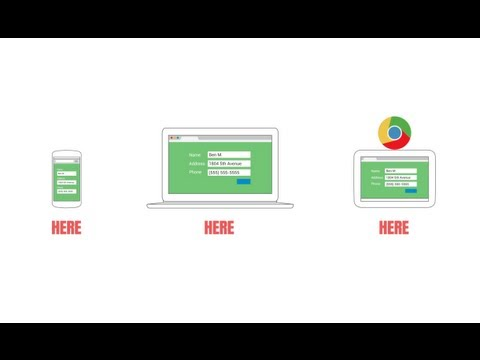
\includegraphics[height=28mm, width=32mm]{images/google.jpg}\\$\;$\\
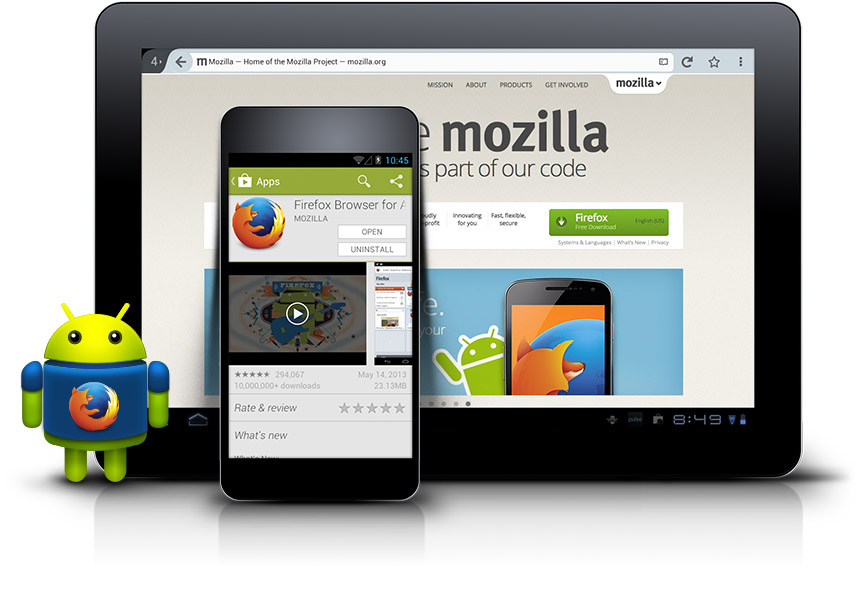
\includegraphics[height=28mm, width=32mm]{images/android-phone-tablet.jpg}
\end{center}
\end{minipage}
\begin{minipage}{.32\linewidth}
\begin{center}
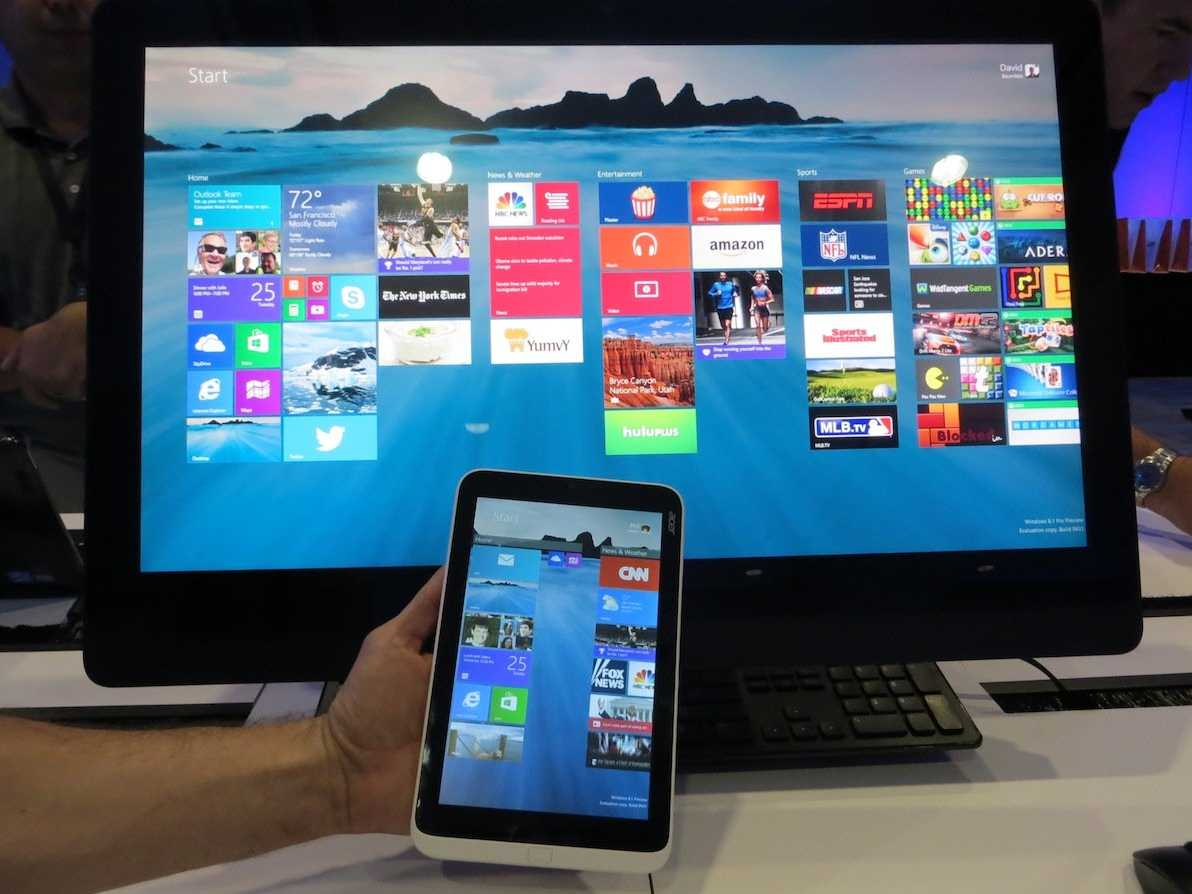
\includegraphics[height=28mm, width=32mm]{images/microsoft1.jpg}\\$\;$\\
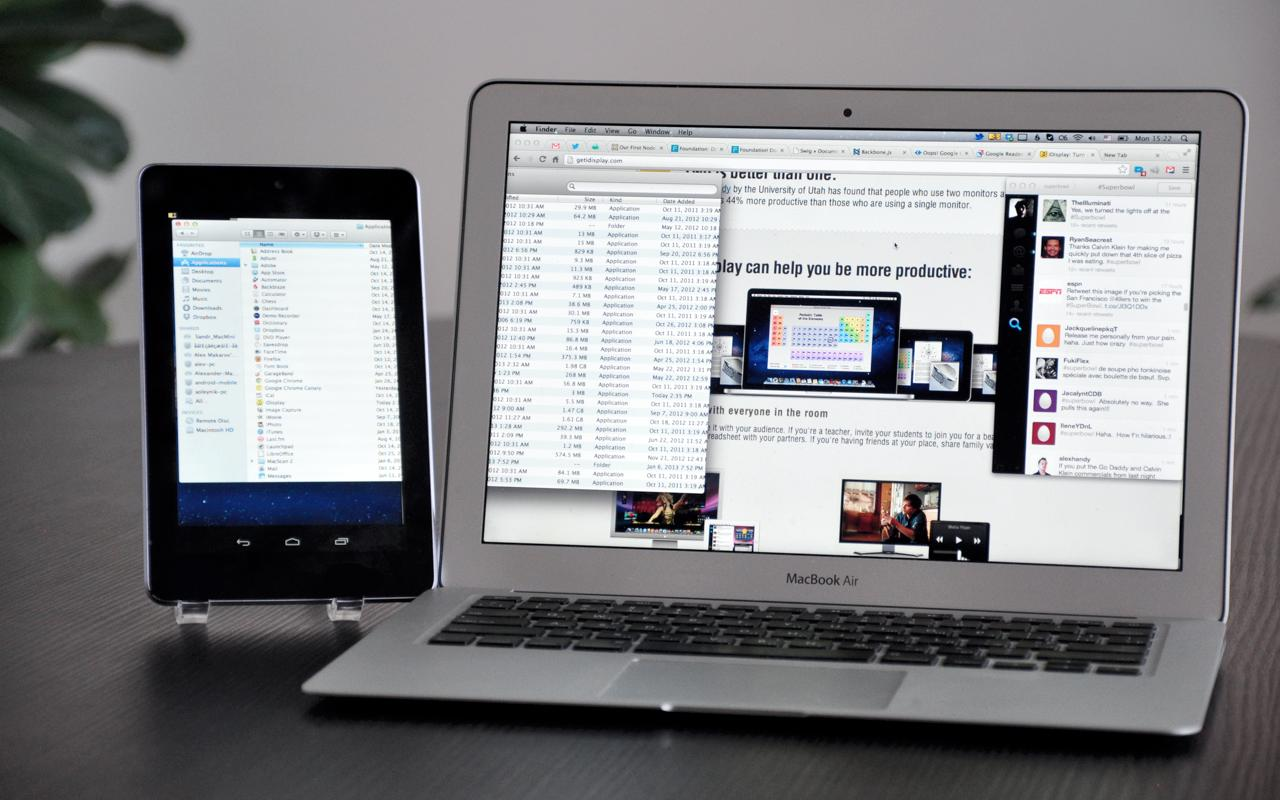
\includegraphics[height=28mm, width=32mm]{images/Apple.jpg}
\end{center}
\end{minipage}
\begin{minipage}{.32\linewidth}
\begin{center}
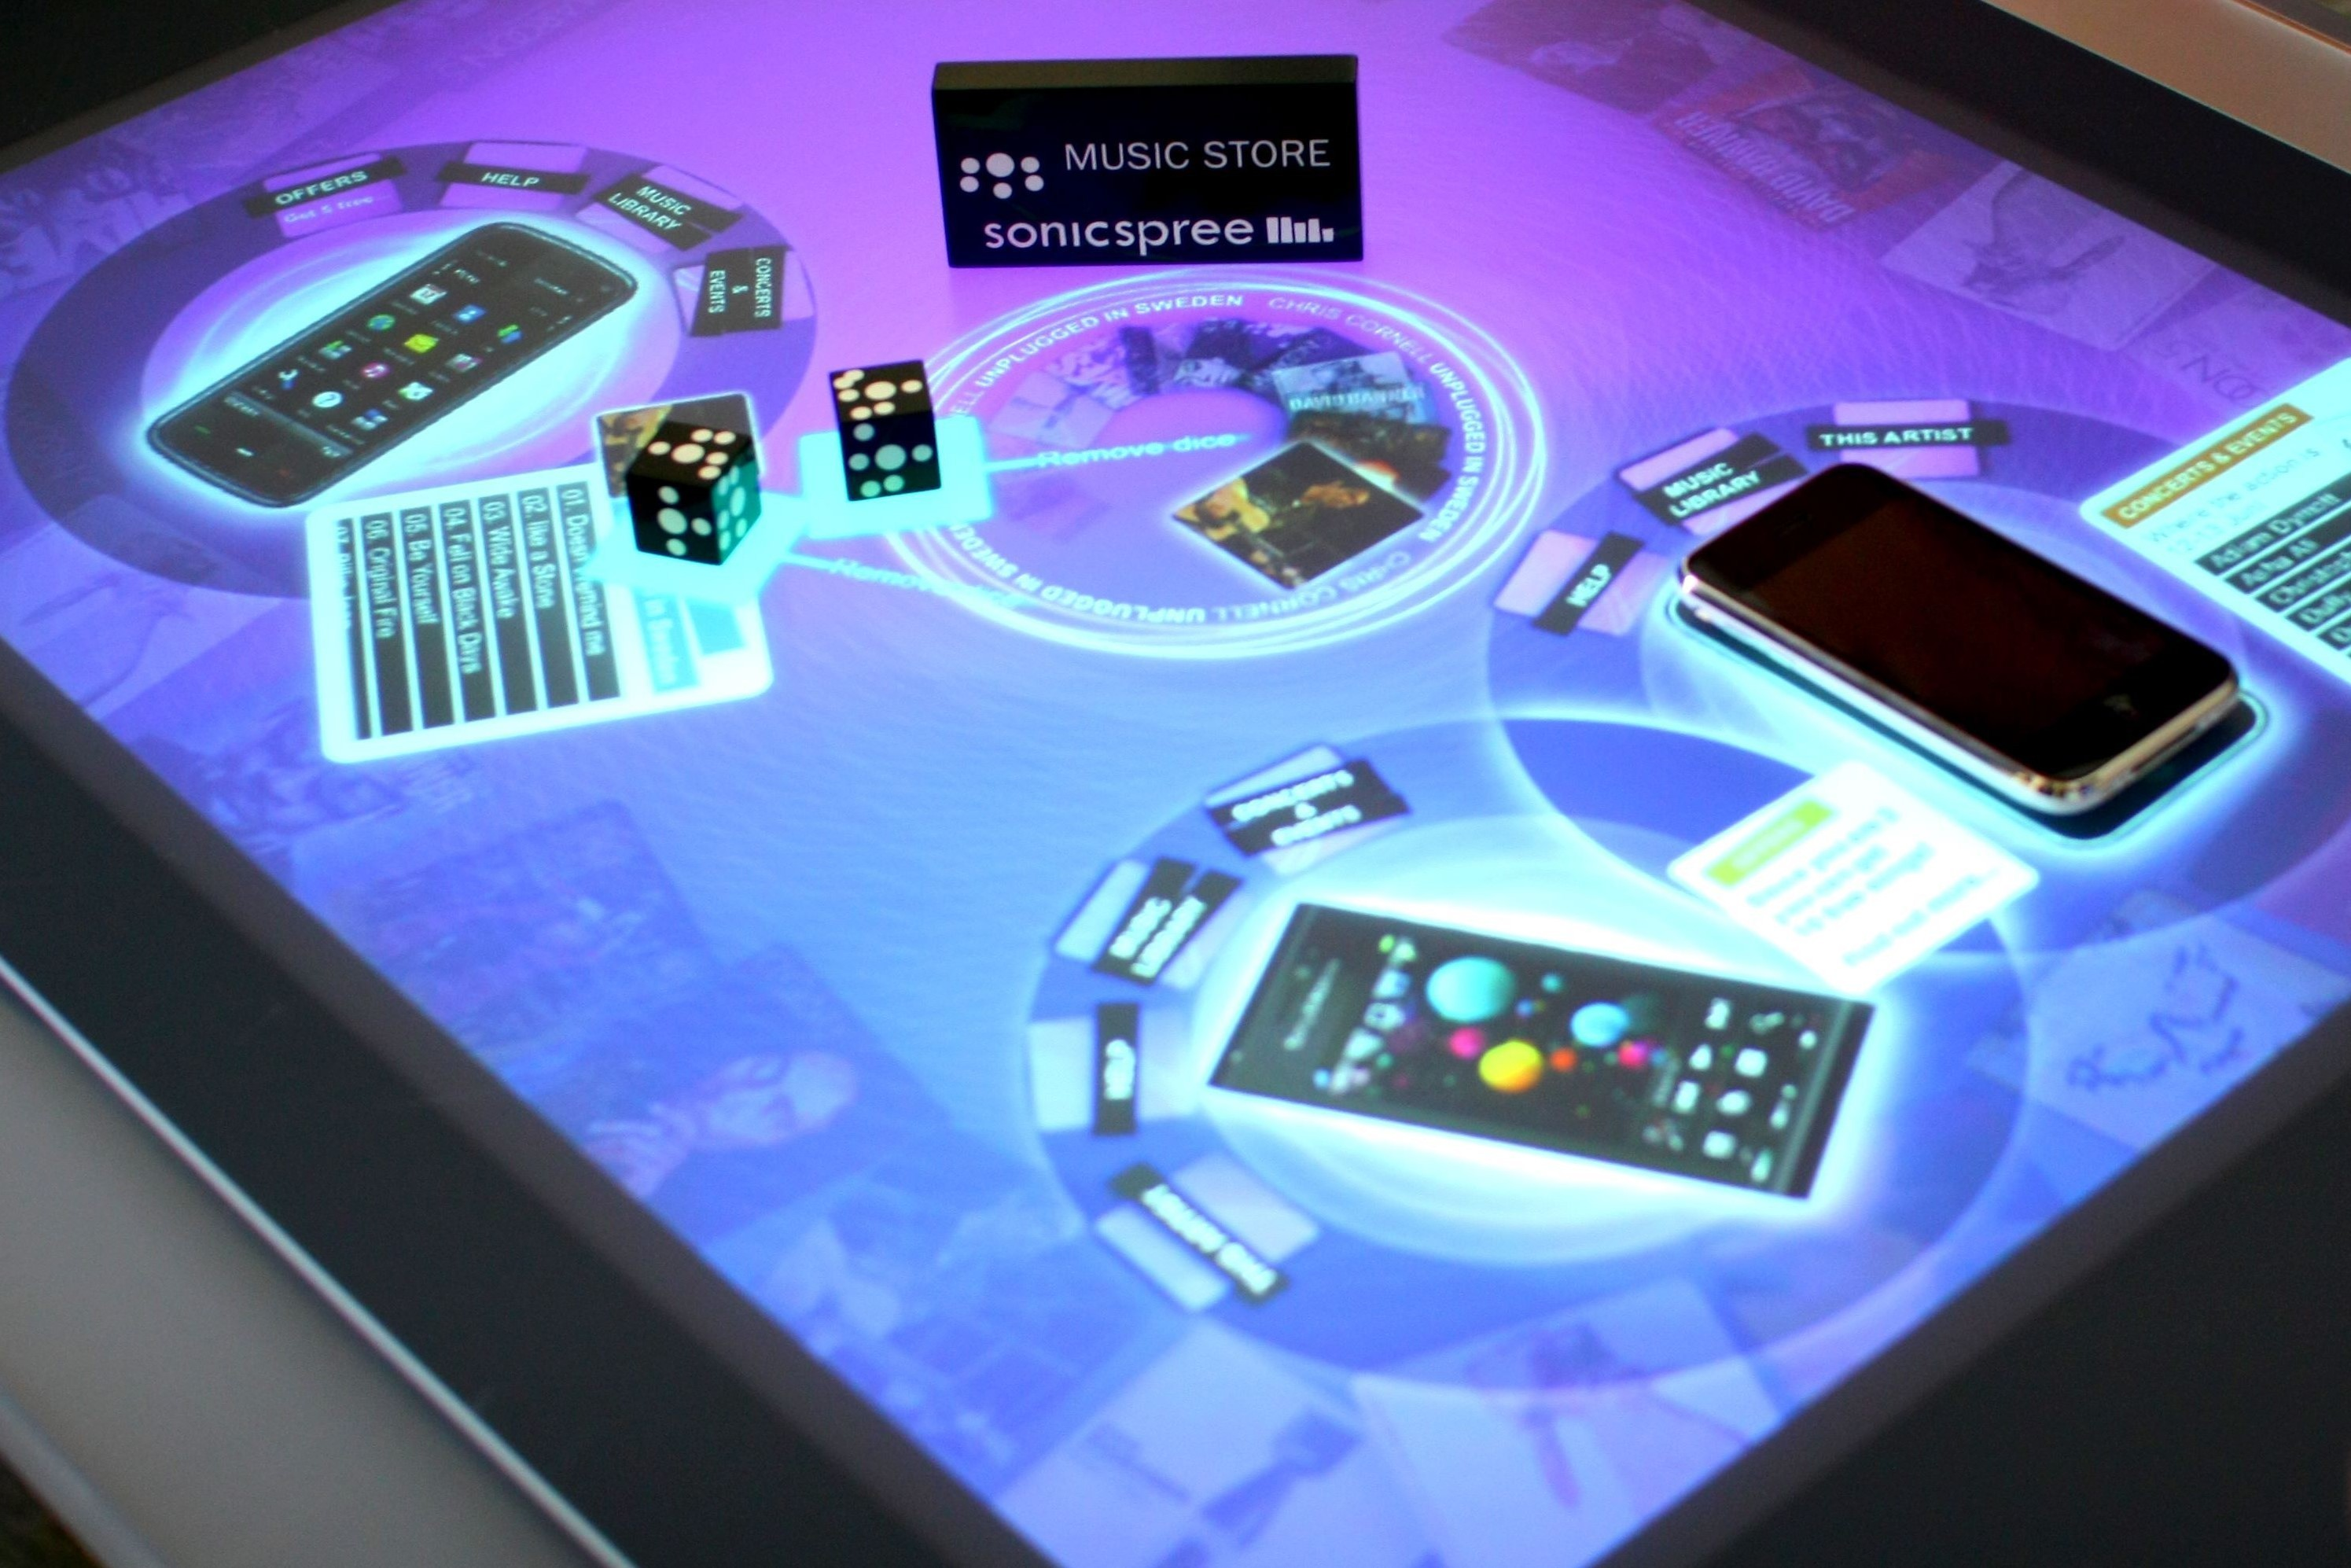
\includegraphics[height=28mm, width=32mm]{images/microsoft2.jpg}\\$\;$\\
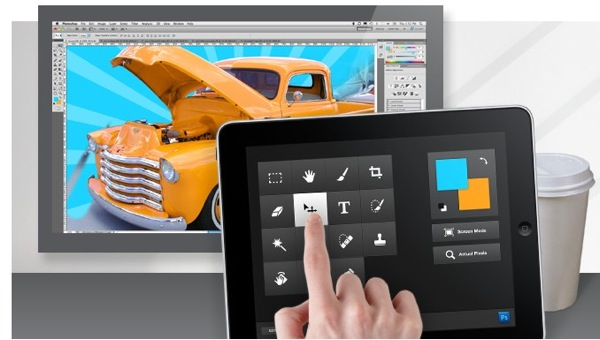
\includegraphics[height=28mm, width=32mm]{images/Adobe.jpg}
\end{center}
\end{minipage}
\end{center}
\end{minipage}
\end{block}
\end{frame}


%\begin{frame}%\frametitle{}
%\begin{block}{Why tui?}
%\begin{minipage}{1.0\linewidth}
%\begin{center}
%\begin{minipage}{.39\linewidth}
%\begin{center}
%Before tui\\$\;$\\
%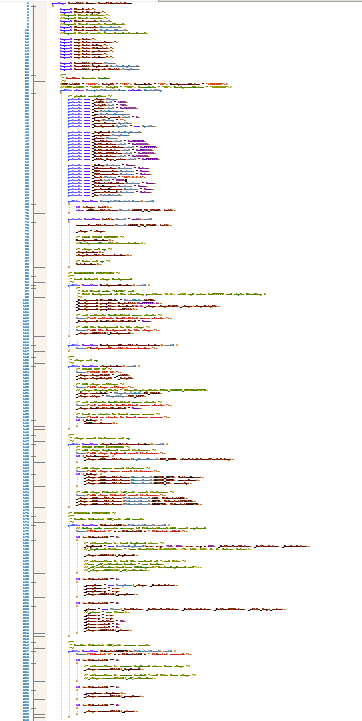
\includegraphics[scale=0.18]{images/old_part1.png}\\
%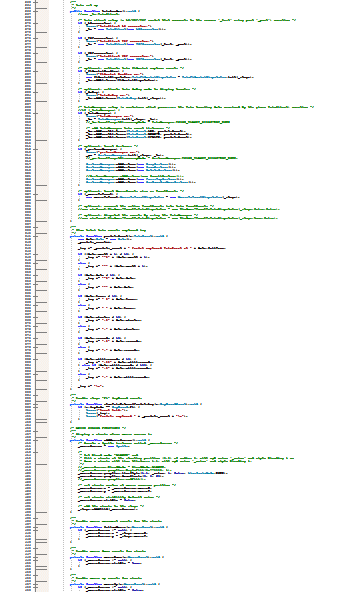
\includegraphics[scale=0.18]{images/old_part2.png}
%\end{center}
%\end{minipage}%\pause
%\begin{minipage}{.59\linewidth}
%\begin{center}
%After tui\\$\;$\\
%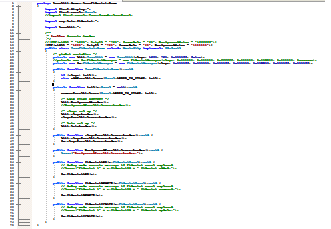
\includegraphics[scale=0.18]{images/new_code.png} 
%\end{center}
%\end{minipage}
%\end{center}
%\end{minipage}
%\end{block}
%\end{frame}
%
%%\begin{frame}%\frametitle{}
%%\begin{block}{Why tui? (cont.)}
%%\begin{minipage}{1.0\linewidth}
%%\begin{center}
%%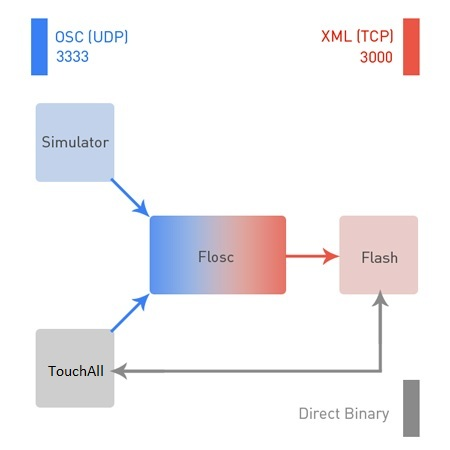
\includegraphics[scale=0.6]{images/flosc.jpg} 
%%\end{center}
%%\end{minipage}
%%\end{block}
%%\end{frame}
%%
%%\begin{frame}%\frametitle{}
%%\begin{block}{Why tui? (cont.)}
%%\begin{minipage}{1.0\linewidth}
%%\begin{center}
%%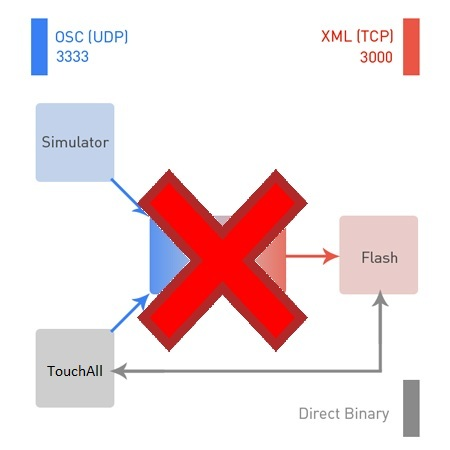
\includegraphics[scale=0.6]{images/no_flosc.jpg} 
%%\end{center}
%%\end{minipage}
%%\end{block}
%%\end{frame}
%
%\begin{frame}%\frametitle{}
%\begin{block}{tui requirements}
%%\begin{block}{Overview (cont.)}
%\begin{minipage}{1.0\linewidth}
%\begin{itemize}
%\item[] 
\includegraphics[scale=0.16]{images/tuioAS3.png}$\;$
%\begin{scriptsize}
%\url{https://goo.gl/FIukmz}
%\end{scriptsize}%\pause
%\item[] 
\includegraphics[scale=0.06]{images/Adobe-Air.jpg}$\;$
%\begin{scriptsize}
%\url{https://goo.gl/FZi1e6}
%\end{scriptsize}
%\item[] 
\includegraphics[scale=0.16]{images/Fx_small.png}$\;$
%\begin{scriptsize}
%\url{https://goo.gl/d3Uw4N}
%\end{scriptsize}%\pause
%\item[] 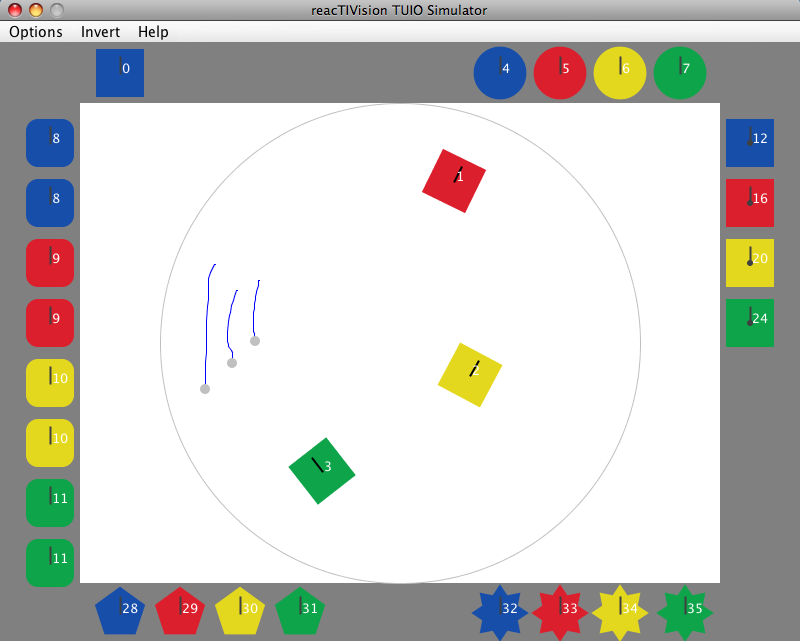
\includegraphics[scale=.08]{images/reactivision04.png}$\;$
%\begin{scriptsize}
%\url{https://goo.gl/YjS2hy}
%\end{scriptsize}
%\item[] 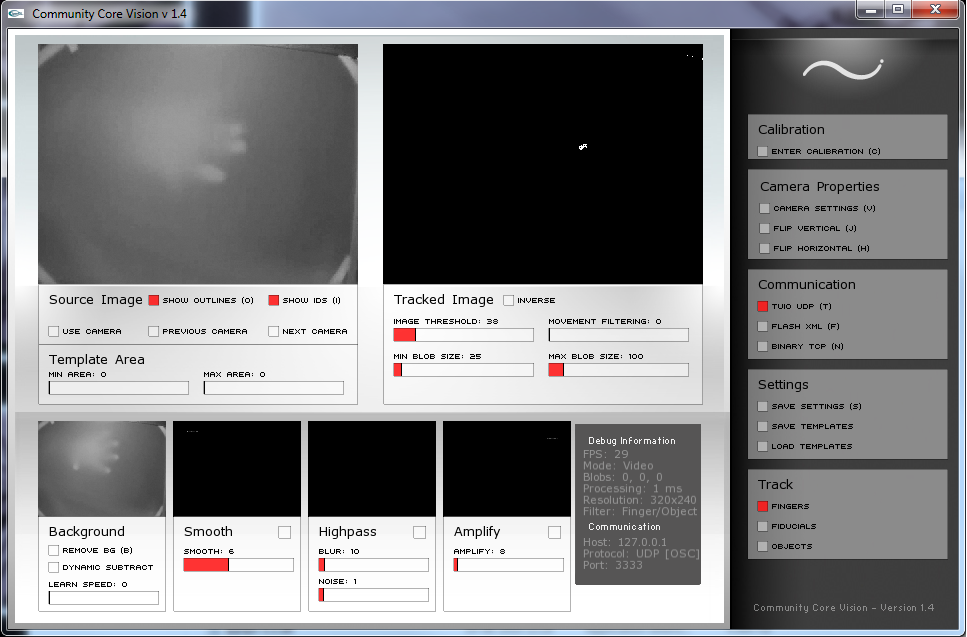
\includegraphics[scale=.09]{images/CCV.png}$\;$
%\begin{scriptsize}
%\url{https://goo.gl/eDPr9z}
%\end{scriptsize}
%\end{itemize}
%\end{minipage}
%\end{block}
%\end{frame}
%
%\begin{frame}%\frametitle{}
%\begin{block}{tui Demos}
%%\begin{block}{Overview (cont.)}
%\begin{minipage}{1.0\linewidth}
%\begin{center}
%\begin{minipage}{.49\linewidth}
%\begin{center}
%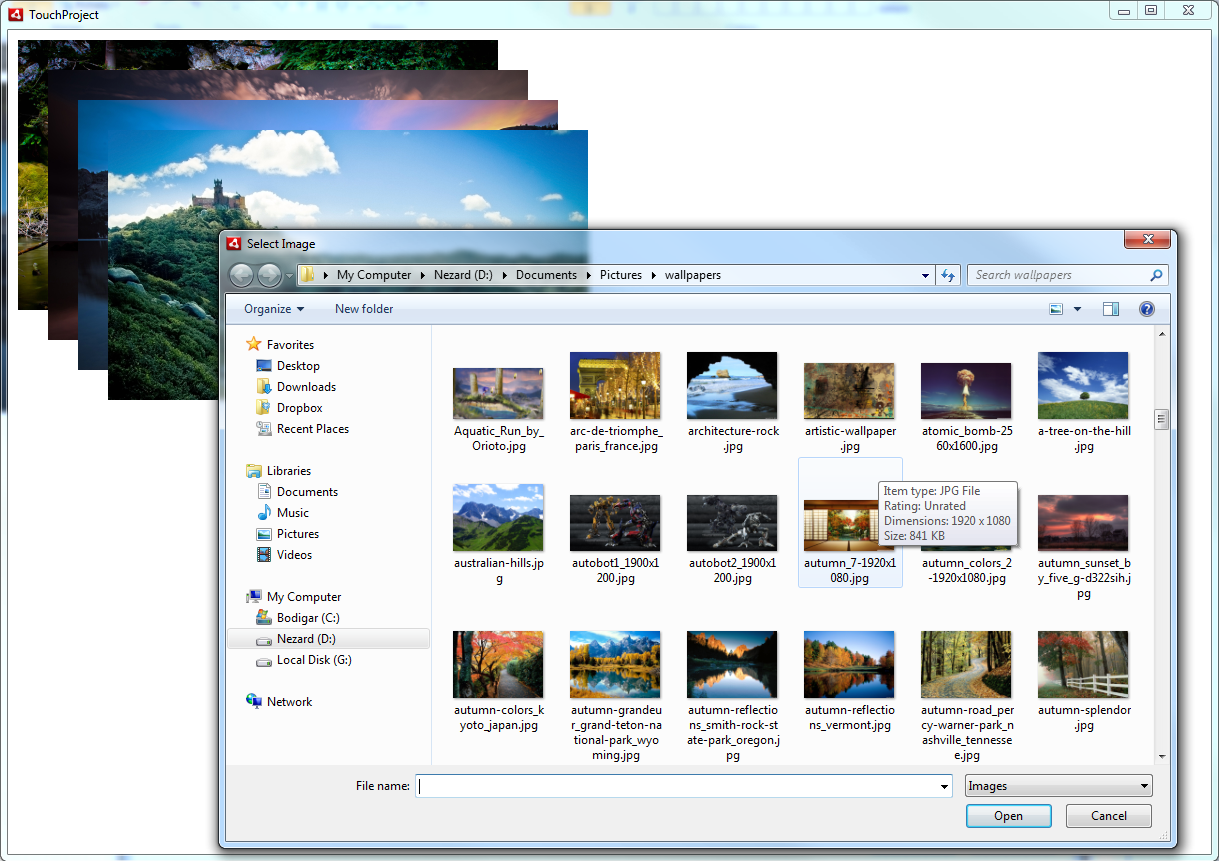
\includegraphics[height=34mm, width=46mm]{images/image_app.png}\\$\;$\\
%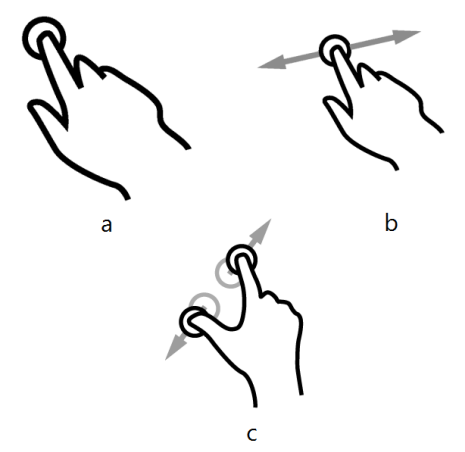
\includegraphics[height=34mm, width=46mm]{images/touch.png}
%\end{center}
%\end{minipage}%\pause
%\begin{minipage}{.49\linewidth}
%\begin{center}
%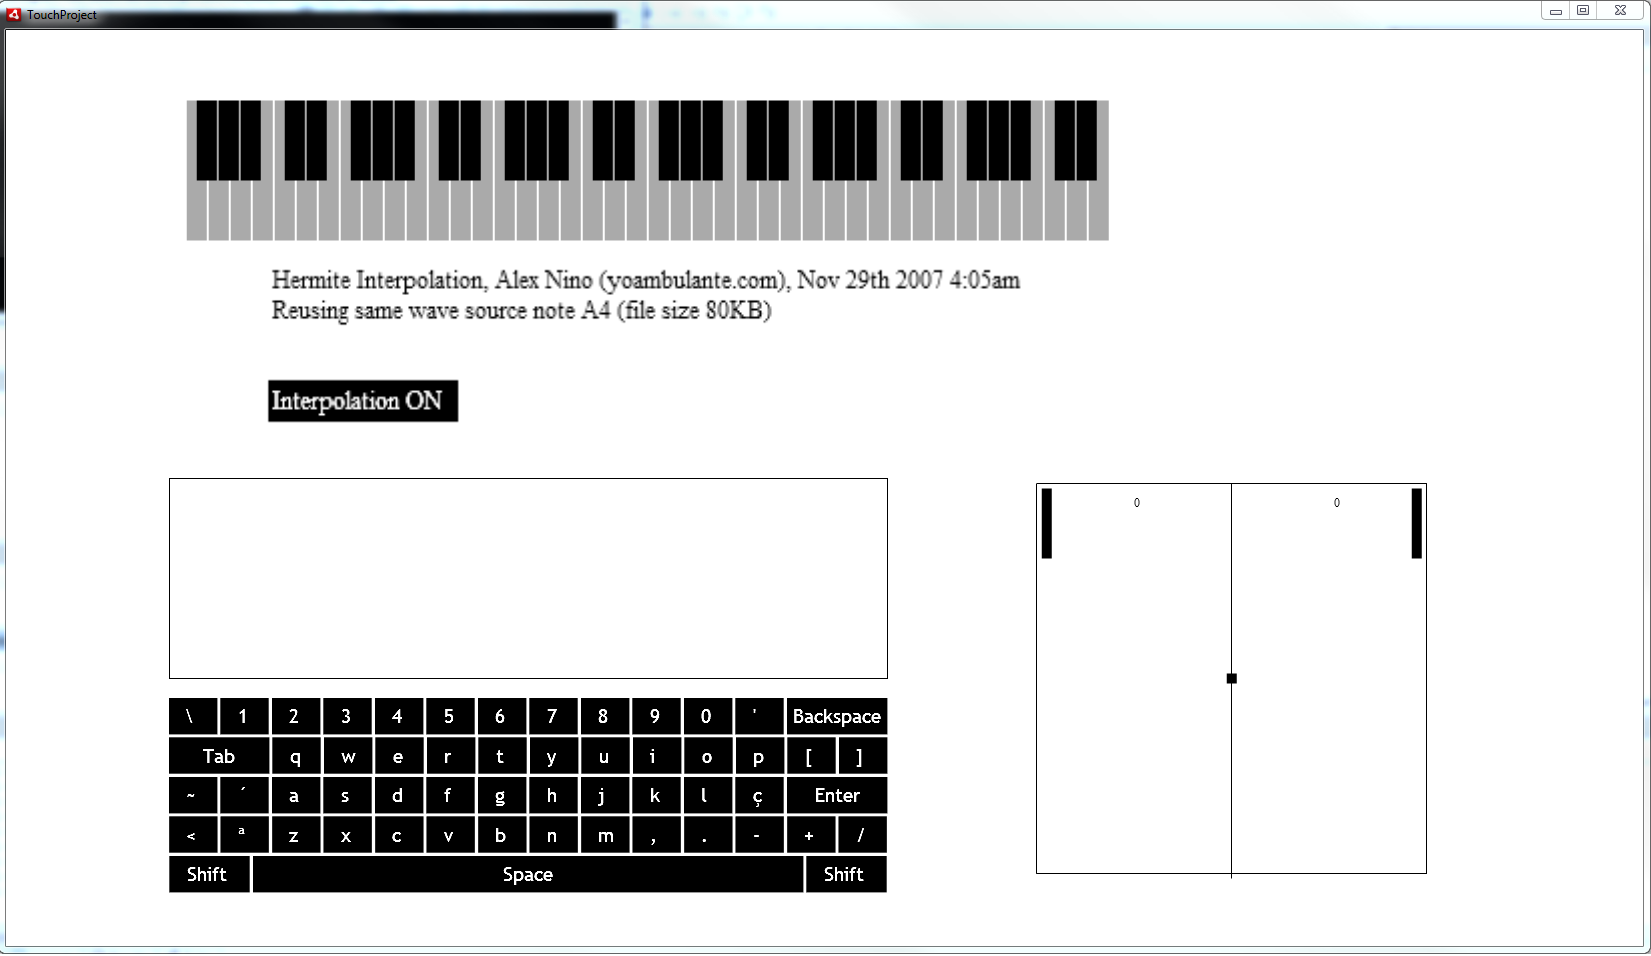
\includegraphics[height=34mm, width=46mm]{images/fiducials.png}\\$\;$\\
%
\includegraphics[height=34mm, width=46mm]{images/fiducial_markers.png} 
%\end{center}
%\end{minipage}
%\end{center}
%\end{minipage}
%\end{block}
%\end{frame}
%
%%\begin{frame}%\frametitle{}
%%\begin{block}{tui App Example}
%%\begin{minipage}{1.0\linewidth}
%%\begin{center}
%%\includemovie[autoclose,text=Click Me!]{100mm}{70mm}{movies/table.avi}
%%\end{center}
%%\end{minipage}
%%\end{block}
%%\end{frame} %5
\section{Building an Optic Touch-table}
\begin{frame}%\frametitle{}
\begin{block}{Building an Optic Touch-table}
\begin{minipage}{1.0\linewidth}
\begin{enumerate}
\item Build Touch-table (MTMini)\\
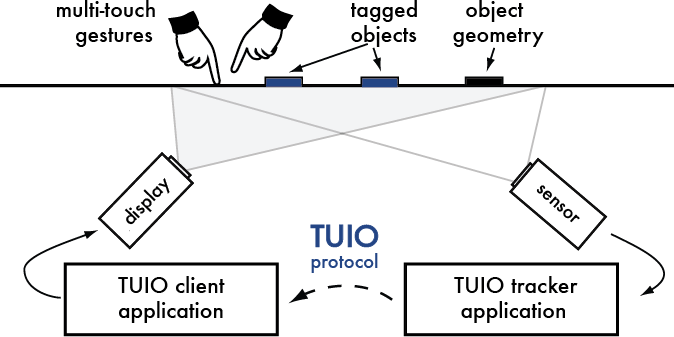
\includegraphics[scale=.19]{images/mesa1.png}\\ 
\url{https://goo.gl/RvtIIv}\\
\url{https://goo.gl/3FO6jB}
\item Add display to multi-touch table (See through LCD Screen)\\
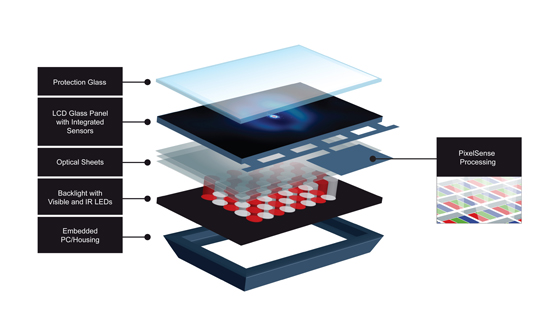
\includegraphics[scale=.19]{images/mesa2.jpg}\\
\url{hhttps://goo.gl/RtLLIr}
%\item Required software\\
%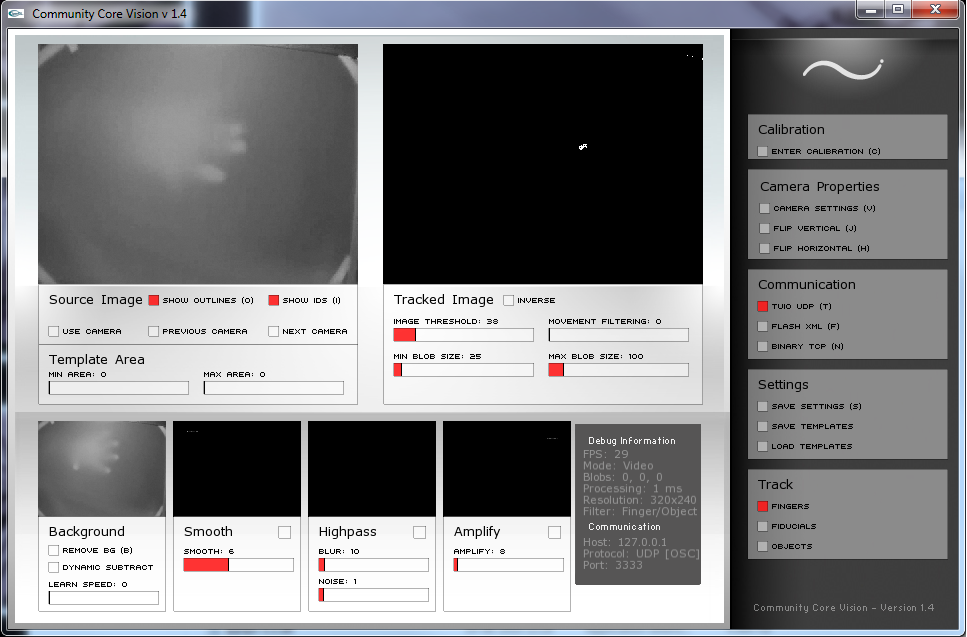
\includegraphics[scale=.09]{images/CCV.png}$\;$\url{https://goo.gl/eDPr9z}
%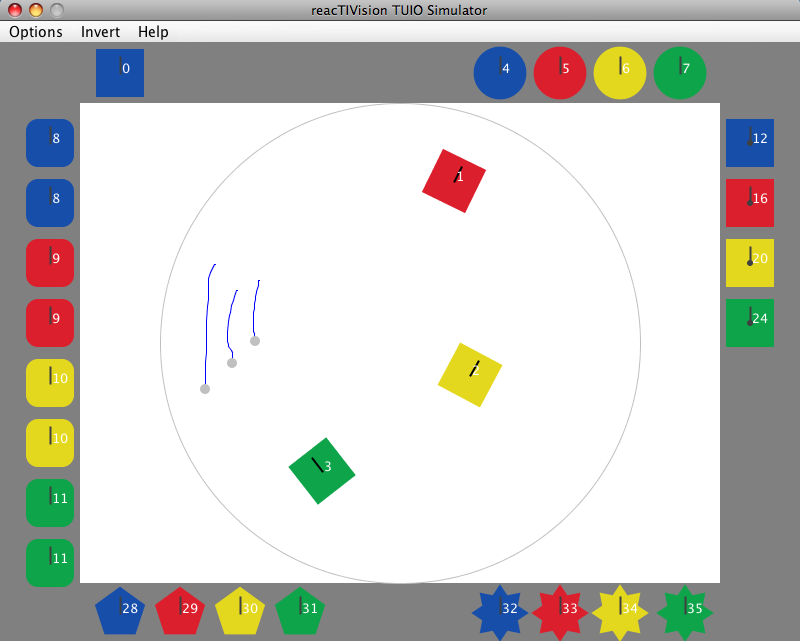
\includegraphics[scale=.08]{images/reactivision04.png}$\;$\url{https://goo.gl/YjS2hy}
\end{enumerate}
\end{minipage}
\end{block}
\end{frame} %1 
\section{TouchAll}
\begin{frame}%\frametitle{}
\begin{block}{Why TUI?}
\begin{minipage}{1.0\linewidth}
\begin{center}
\begin{minipage}{.39\linewidth}
\begin{center}
Before TUI\\$\;$\\
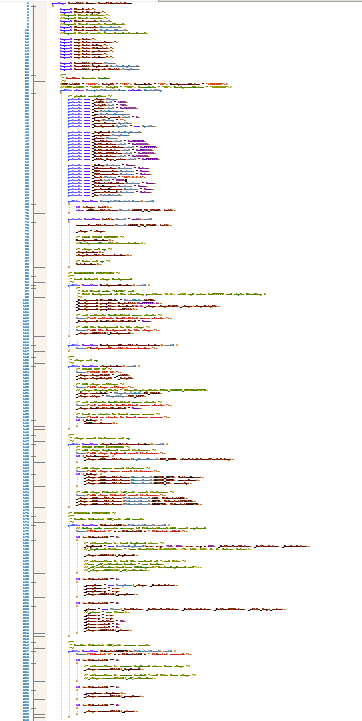
\includegraphics[scale=0.18]{images/old_part1.png}\\
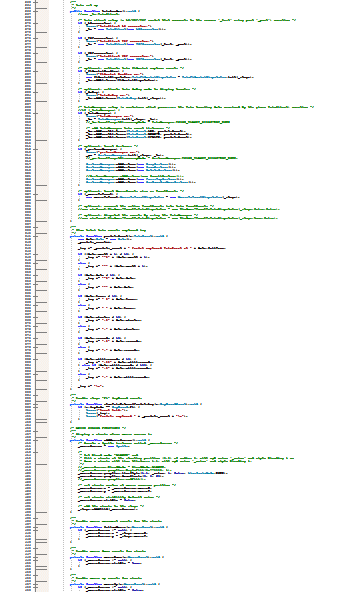
\includegraphics[scale=0.18]{images/old_part2.png}
\end{center}
\end{minipage}%\pause
\begin{minipage}{.59\linewidth}
\begin{center}
After TUI\\$\;$\\
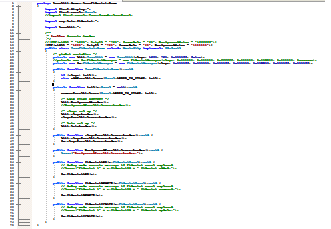
\includegraphics[scale=0.18]{images/new_code.png} 
\end{center}
\end{minipage}
\end{center}
\end{minipage}
\end{block}
\end{frame}

%\begin{frame}%\frametitle{}
%\begin{block}{Why TUI? (cont.)}
%\begin{minipage}{1.0\linewidth}
%\begin{center}
%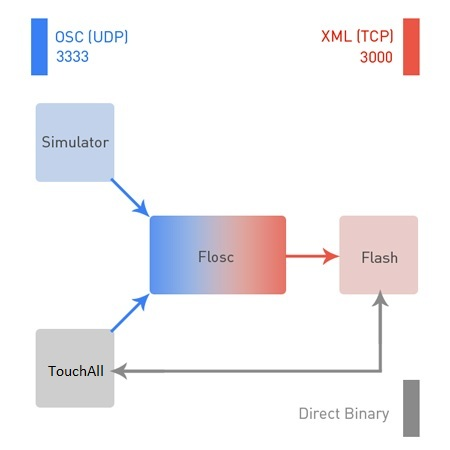
\includegraphics[scale=0.6]{images/flosc.jpg} 
%\end{center}
%\end{minipage}
%\end{block}
%\end{frame}
%
%\begin{frame}%\frametitle{}
%\begin{block}{Why TUI? (cont.)}
%\begin{minipage}{1.0\linewidth}
%\begin{center}
%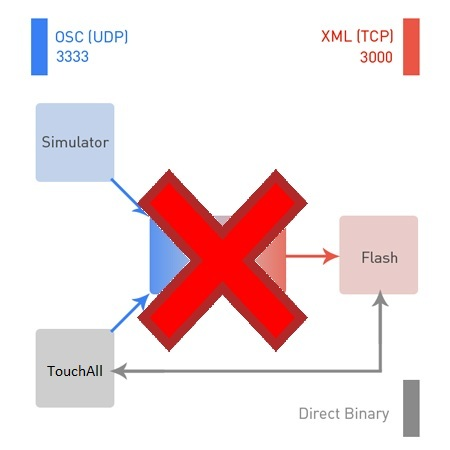
\includegraphics[scale=0.6]{images/no_flosc.jpg} 
%\end{center}
%\end{minipage}
%\end{block}
%\end{frame}

\begin{frame}%\frametitle{}
\begin{block}{TUI requirements}
%\begin{block}{Overview (cont.)}
\begin{minipage}{1.0\linewidth}
\begin{itemize}
\item[] 
\includegraphics[scale=0.16]{images/tuioAS3.png}$\;$
\begin{scriptsize}
\url{https://goo.gl/FIukmz}
\end{scriptsize}%\pause
\item[] 
\includegraphics[scale=0.16]{images/Adobe-Air.jpg}$\;$
\begin{scriptsize}
\url{https://goo.gl/FZi1e6}
\end{scriptsize}
\item[] 
\includegraphics[scale=0.16]{images/Fx_small.png}$\;$
\begin{scriptsize}
\url{https://goo.gl/d3Uw4N}
\end{scriptsize}%\pause
\item[] 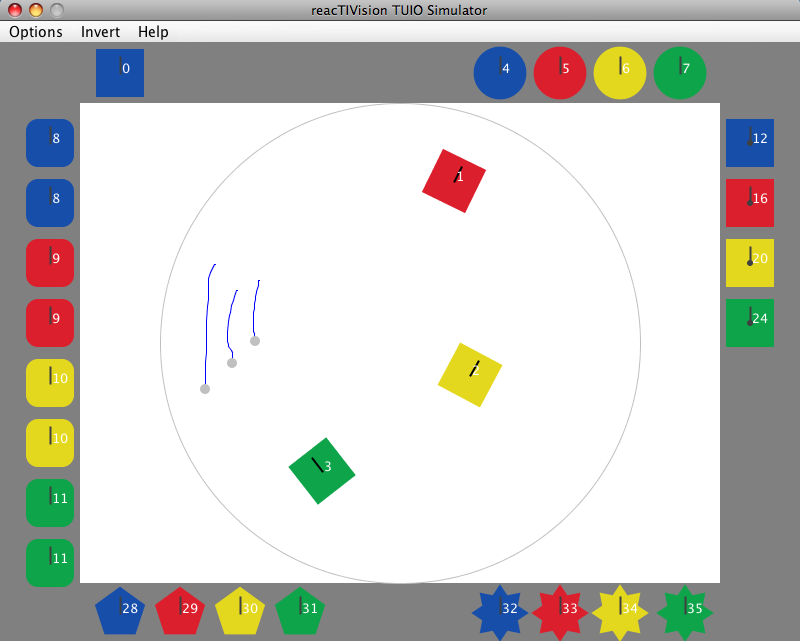
\includegraphics[scale=.08]{images/reactivision04.png}$\;$
\begin{scriptsize}
\url{https://goo.gl/YjS2hy}
\end{scriptsize}
\item[] 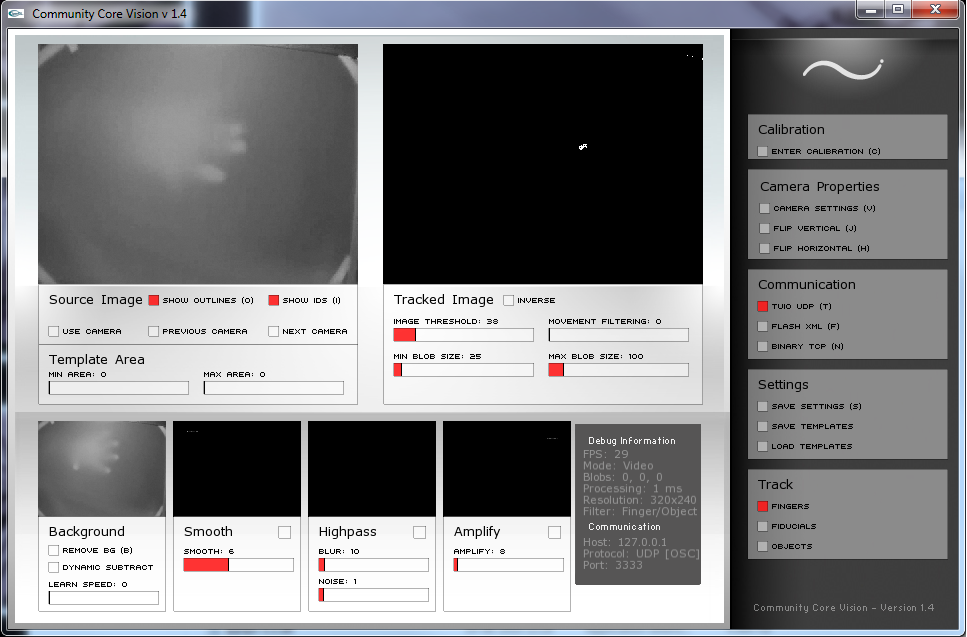
\includegraphics[scale=.09]{images/CCV.png}$\;$
\begin{scriptsize}
\url{https://goo.gl/eDPr9z}
\end{scriptsize}
\end{itemize}
\end{minipage}
\end{block}
\end{frame}

\begin{frame}%\frametitle{}
\begin{block}{TUI architecture}
%\begin{block}{TUI, TUIO AS3, and Flex and Air SDKs layers diagram}
\begin{minipage}{1.0\linewidth}
\begin{center}
\begin{minipage}{.49\linewidth}
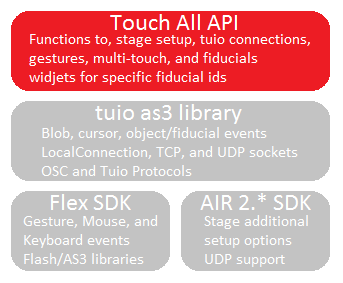
\includegraphics[height=70mm, width=45mm]{images/API&tuioas3lib&skds.png}$\;$ 
%\end{center}
\end{minipage}
%\end{block}
%\end{frame}
%
%\begin{frame}%\frametitle{}
%\begin{block}{TUI and TUIO AS3 modules}
%\begin{minipage}{1.0\linewidth}
\begin{minipage}{.49\linewidth}
%\begin{center}
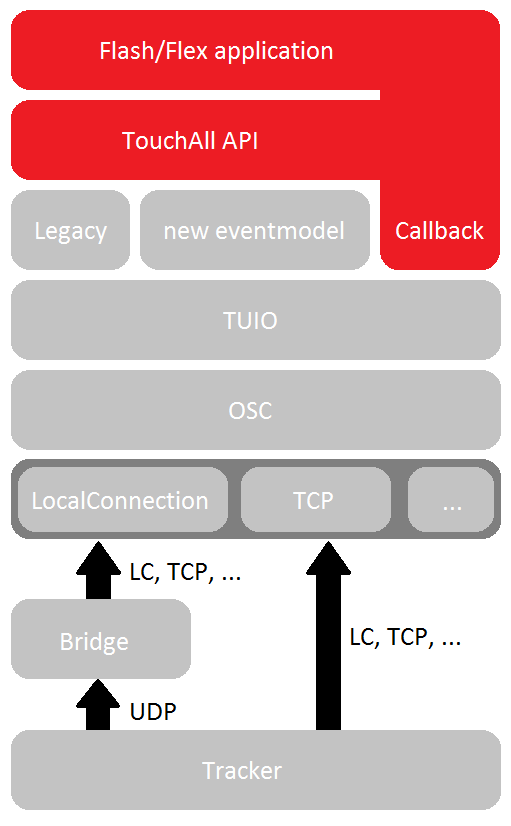
\includegraphics[scale=0.33]{images/as3LibDiagram.png} 
%\end{center}
\end{minipage}
\end{center}
\end{minipage}
\end{block}
\end{frame}

%\begin{frame}%\frametitle{}
%\begin{block}{TUI and TUIO AS3 modules}
%\begin{minipage}{1.0\linewidth}
%\begin{center}
%\includemovie[autoclose,text=Click Me!]{100mm}{70mm}{movies/app.avi}
%\end{center}
%\end{minipage}
%\end{block}
%\end{frame}

\begin{frame}%\frametitle{}
\begin{block}{TUI Demos}
%\begin{block}{Overview (cont.)}
\begin{minipage}{1.0\linewidth}
\begin{center}
\begin{minipage}{.49\linewidth}
\begin{center}
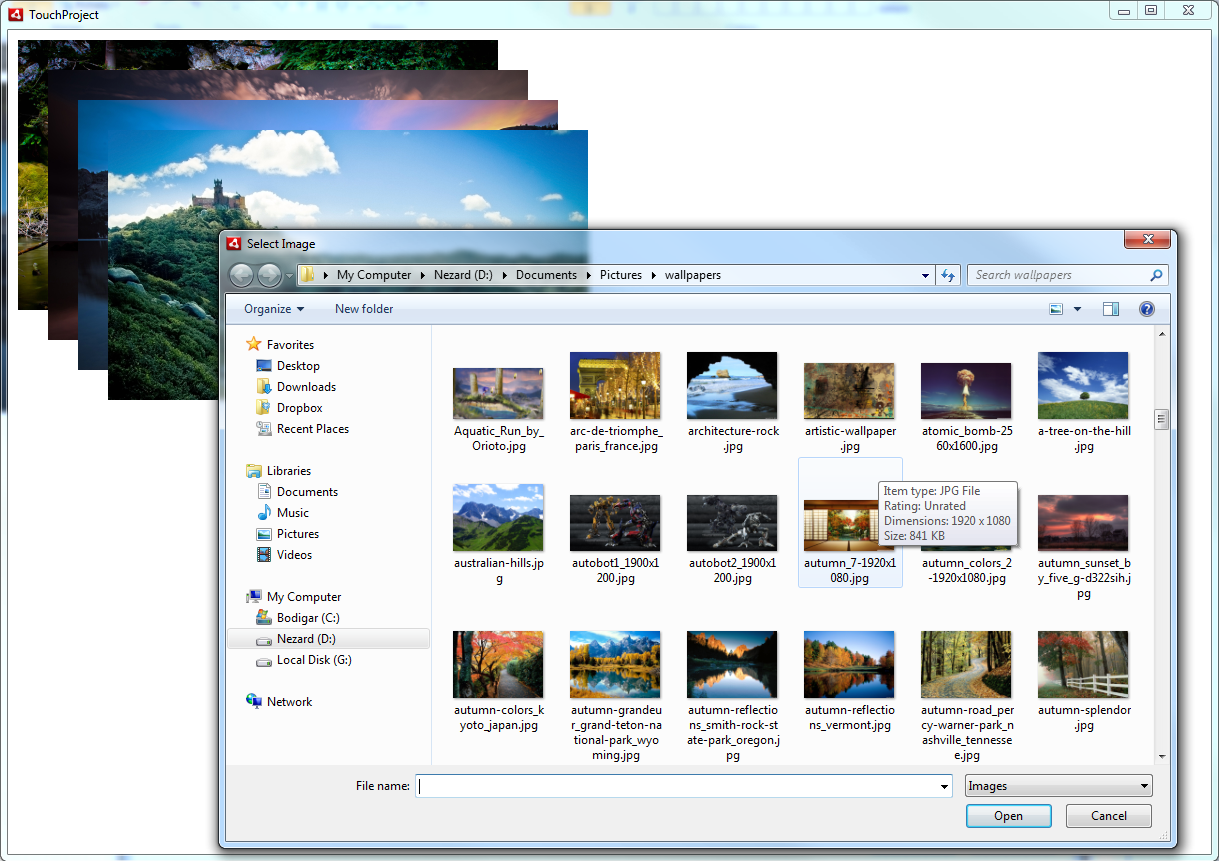
\includegraphics[height=34mm, width=46mm]{images/image_app.png}\\$\;$\\
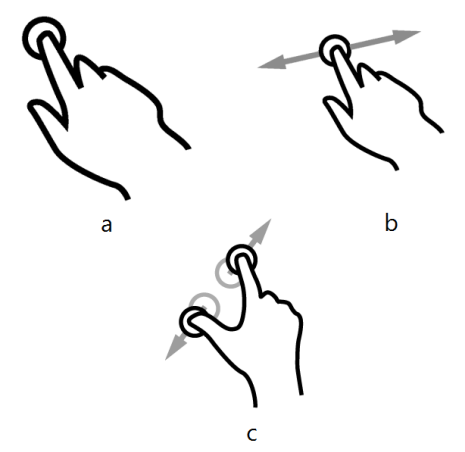
\includegraphics[height=34mm, width=46mm]{images/touch.png}
\end{center}
\end{minipage}%\pause
\begin{minipage}{.49\linewidth}
\begin{center}
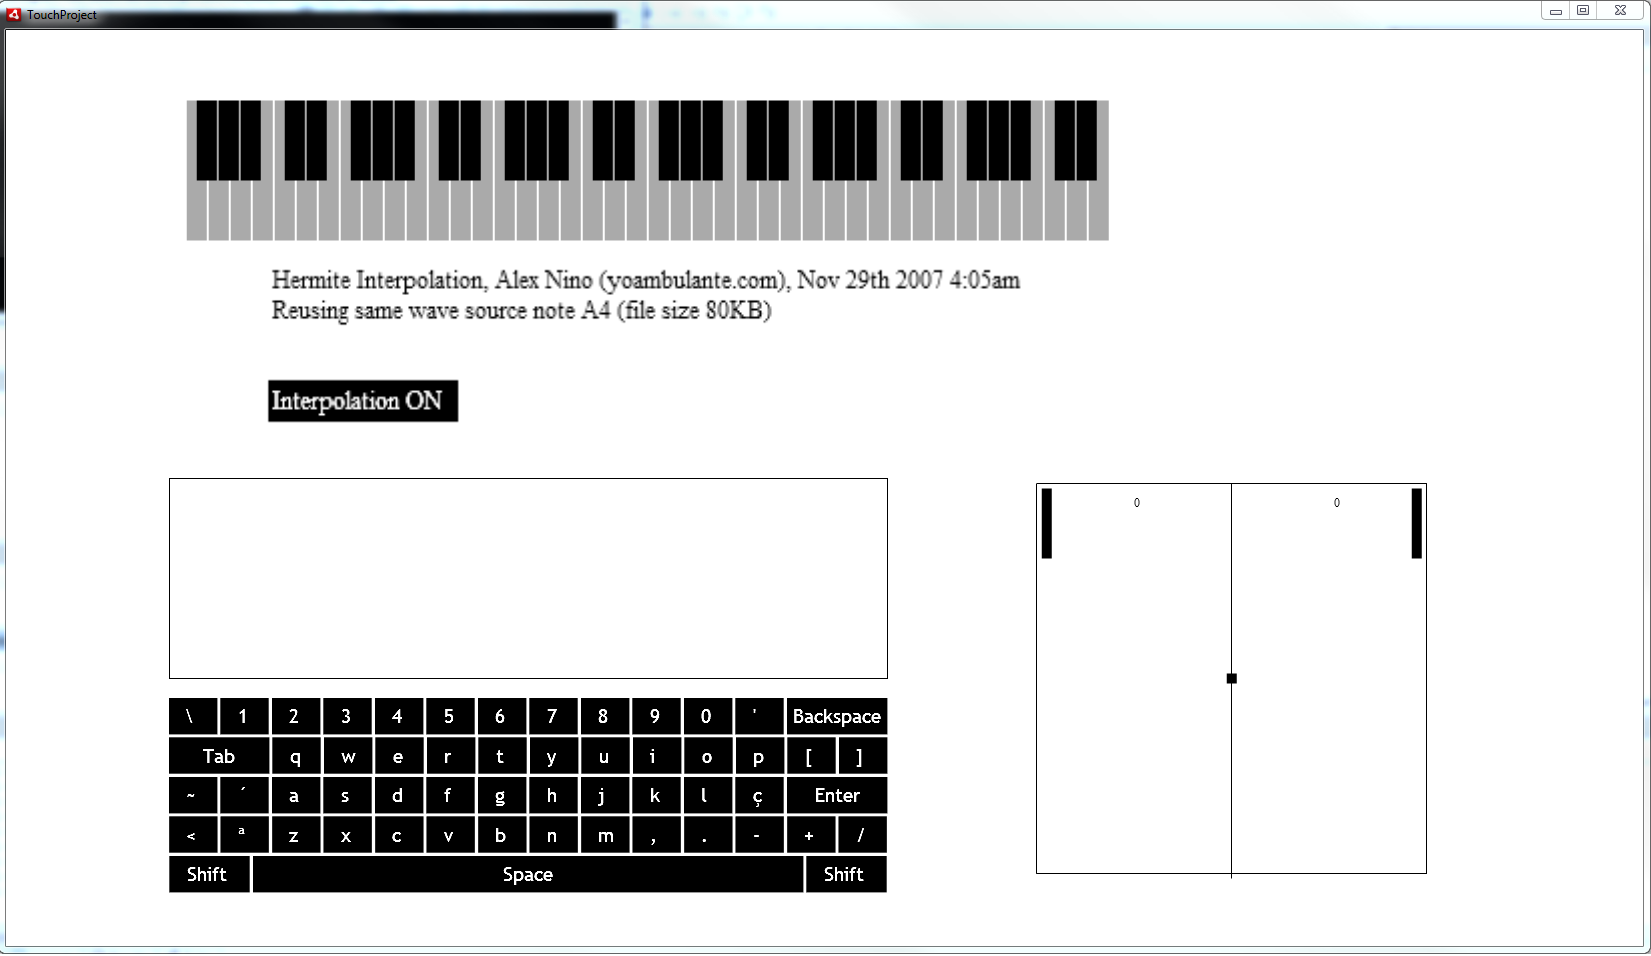
\includegraphics[height=34mm, width=46mm]{images/fiducials.png}\\$\;$\\

\includegraphics[height=34mm, width=46mm]{images/fiducial_markers.png} 
\end{center}
\end{minipage}
\end{center}
\end{minipage}
\end{block}
\end{frame}

%\begin{frame}%\frametitle{}
%\begin{block}{TUI App Example}
%\begin{minipage}{1.0\linewidth}
%\begin{center}
%\includemovie[autoclose,text=Click Me!]{100mm}{70mm}{movies/table.avi}
%\end{center}
%\end{minipage}
%\end{block}
%\end{frame} %3 
%\section{UDP VS TCP Networking Analysis}
\begin{frame}%\frametitle{}
\begin{block}{UDP VS TCP Networking Analysis}
\begin{table}
\centering
\small
\begin{tabular}{|>{\centering}p{1.4cm}<{\centering}|c|c|>{\centering}p{1.4cm}|p{1.6cm}<{\centering}|}
\hline
& & & \textbf{Packet} & \textbf{Average} \\
\textbf{Protocol} & \textbf{First Packet} & \textbf{Last Packet} & \textbf{Transfer} & \textbf{Packets}\\
& \textbf{Sent Date} & \textbf{Arrival Date} & \textbf{Time (ms)} & \textbf{Captured}\\
\hline
UDP & 2011-02-17 & 2011-02-17 & 14.957 & 70\\ 
& 10:57:31.357 & 10:57:31.837 & & \\ 
\hline
TCP & 2011-02-17 & 2011-02-17 & 16.100 & 80\\
& 11:01:03.818 & 11:01:41.616 & & \\
\hline
\end{tabular}
\end{table}
\end{block}
\end{frame} %1
\section{Conclusions}
\begin{frame}%\frametitle{}
\begin{block}{Conclusions}
\begin{itemize}
\begin{minipage}{.9\linewidth} 
%\item Previous solutions using a bridge took more time due to TCP to UDP datagram conversion.
\item The time required in developing applications for multi-touch devices can be shortened using tui.\\
\item tui allows to use fiducials and multi-touch through UDP, TCP, flash LocalConnection all in once. \\
\item ActionbScript-based non-free software alternatives exist, but not with native fiducial support. 
\end{minipage}
\end{itemize}
\end{block}
\end{frame}

\begin{frame}%\frametitle{}
\begin{block}{Future work}
\begin{itemize}
\begin{minipage}{.9\linewidth} 
\item Development of tools that allow device emulation, for multi-touch, multi-mouse pointer, and platform independent application testing.\\
\item Include in the tui more native widgets for specific fiducials.\\
\item Include in the tui support for 3D object loading and gesture based manipulation.\\
\item Integrate the tui as a module of an 2D/3D ActionScript 3.0 game engine.
\end{minipage}
\end{itemize}
\end{block}
\end{frame}

\begin{frame}%\frametitle{}
\begin{block}{}
\begin{center}
Questions, Comments, Observations, \\
Twitter twitts, Facebook like's/posts/comments???
\end{center}
\end{block}
\end{frame} %3 (i.e., 2) 
\end{document}